\documentclass{article}
\usepackage[utf8]{inputenc}
\usepackage{amsmath}
\usepackage{amssymb}
\usepackage{amsfonts}
\usepackage[dvipsnames]{xcolor}
\usepackage{listings}
\usepackage{graphicx}
\setlength{\parskip}{03pt} 
\setlength{\textheight}{ 620 pt}
\setlength{\voffset}{-20 pt}
\setlength{\headsep}{12 pt}
\setlength{\headheight}{14 pt}
\setlength{\topskip}{12 pt}
\setlength{\footskip}{30 pt}
\usepackage{fancyhdr}
\pagestyle{fancy}
\newcommand{\bs}[1]{\boldsymbol{#1}}

\fancyhead{}

\fancyhead[L]{\textbf{Esha Chakrabarty}} % TYPE YOUR NAME HERE!
\fancyhead[R]{\textbf{920884665}}
%%%%%%%%%%%%%%%%%%%%%%%%%%%%%%%%%%%%%% TITLE, AUTHOR AND DATE %%%%%%%%%%%%%%%%%%%%%%%%%%%%%%%%%%%%%%

\title{MAT 167 WQ 2024 CA 01 Report}
\author{Esha Chakrabarty}
\date{\today}

\begin{document}

\maketitle
\tableofcontents
\newpage

\section{Introduction and Motivation}

In this exercise we use DCT (Discrete Cosine Transformation) in order to compress an audio signal. In the real world, this signal can be $10^16$ points long; however for the purposes of this exercise we use a very small signal.  

This is important because the transformation and compression techniques we used are crucial to music streaming services which is the primary form of audio consumption today. Audio frequencies are taken and optimized in order to preserve the sound but compress the amount of data required to relay that message.

Throughout this exercise I was able to learn that even though using the full signal vector is most accurate, it is possible to create a similar level of accuracy by only using the largest “weights” or values in the vector $\bs{a}$

\subsection{Professor Saito's Notes}

Any vector $\bs{x}$ of length $n$ can be represented as the product of an $n \times n$ elementary matrix and a vector of coefficients containing {$x_1, x_2, … x_n$}. This method uses the standard, or canonical, basis. However, this is not always the most efficient way to represent a vector. We can create a matrix $U$ that forms a DCT basis in $\mathbb{R}^n$ in place of the elementary matrix. Then, rather than using the $x$ values already present in $\bs{x}$ we can derive a new vector $\bs{a}$ that contains the coefficient values $a_1, a_2, … a_n$
$$\bs{x} =E\bs{x} = U\bs{a}$$
This method using DCT is normally better for the typical musical signal and there is an audible difference from using the canonical basis.

\section{Data Set}

$\bs{x}$ is a signal vector that represents a very short audio signal. 

The matrix $U$ is the result of the Discrete Cosine Transformation that forms a basis in $\mathbb{R}^8$. There was a given $U$ matrix in the original file however I am using the matrix obtained from the DCT formula 
$$\cos\left(\frac{k \pi (x - 1)}{7}\right)$$
 and my modified Gram-Schmidt program for orthonormalization.

It is unclear exactly how the data for $\bs{x}$ was obtained however it could be a snippet of an audio recording. 

\section{Procedure}

In order to perform this exercise we begin by visualizing the signal. We then derive the DCT formulas and create a matrix $A$. Then we orthonormalize the matrix to derive $U$. We use the formula $\bs{a} = U^T\bs{x}$ in order to find the vector $\bs{a}$. Finally we choose the largest (most influential) values of $\bs{a}$ in order to reconstruct an approximation of $\bs{x}$ using the equation $\bs{x}_i = U\bs{a}_i$ Lastly, we experiment with varying degrees of compression to optimize the amount of data and relative error. 

\subsection{Loading and Understanding the Data}

\begin{figure}[h!]
	\centering
	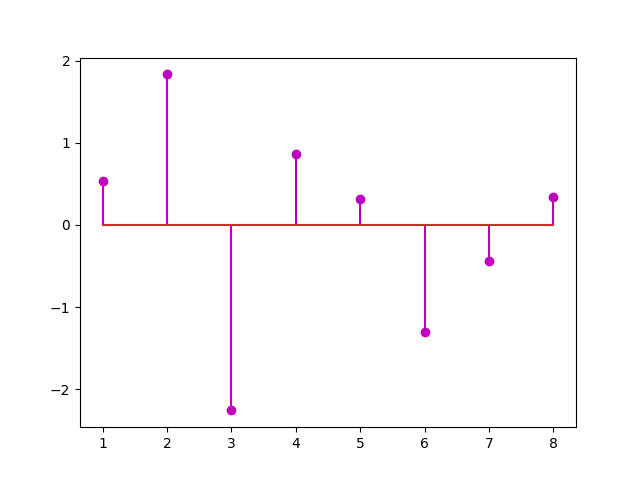
\includegraphics[scale=0.5]{CA_01Figure_1.png}
	\caption{Signal $\bs{x}$}
	\label{fig: FIG 01}
\end{figure}

Visualization of the audio signal $\bs{x}$ of 8 samples.

\subsection{Finding Orthonormal Basis Vectors}

\begin{figure}[h!]
	\centering
	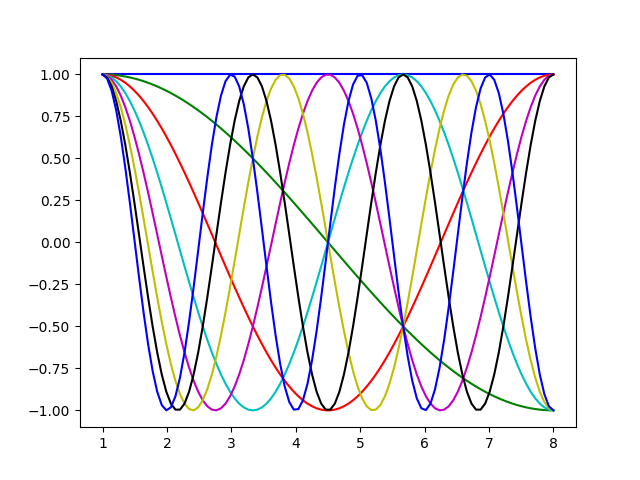
\includegraphics[scale=0.5]{CA_01Figure_2.png}
	\caption{The functions $f_k(x)$ plotted}
	\label{fig: FIG 02}
\end{figure}

Visualization of the 8 continuous functions on the interval 1 to 8 where $k = 0...7$. We then input $\bs{x}$ into each of these functions to create an $8 \times 8$ matrix. 

$$ A = \begin{bmatrix}
	1 & 1 & 1 & 1 & 1 & 1 & 1 & 1 \\
	1 & 0.9010 & 0.6235 & 0.2225 & -0.2225 & -0.6235 & -0.9010 & -1 \\
	1 & 0.6235 & -0.2225 & -0.9010 & -0.9010 & -0.2225 & 0.6235 & 1 \\
	1 & 0.2225 & -0.9010 & -0.6235 & 0.6235 & 0.9010 & -0.2225 & -1 \\
	1 & -0.2225 & -0.9010 & 0.6235 & 0.6235 & -0.9010 & -0.2225 & 1 \\
	1 & -0.6235 & -0.2225 & 0.9010 & -0.9010 & 0.2225 & 0.6235 & -1 \\
	1 & -0.9010 & 0.6235 & -0.2225 & -0.2225 & 0.6235 & -0.9010 & 1 \\
	1 & -1 & 1 & -1 & 1 & -1 & 1 & -1 \\
	\end{bmatrix} $$

However, the column vectors of $A$ are not orthonormal. We know this because $A^TA \neq I$. If A was orthonormal then $A^TA$ would equal the identity matrix. Rather than use the provided $U$ matrix, I used my modified Gram-Schmidt program in order to create an orthonormal basis for $\mathbb{R}^8$

$$ U = \begin{bmatrix}
	 0.3536 & 0.4714 & 0.4183 & 0.3761 & 0.3416 & 0.3129 & 0.2887 & 0.1961 \\
	0.3536 & 0.4247 & 0.2383 & 0.0108 & -0.2182 & -0.4070 & -0.5202 & -0.3922 \\
	0.3536 & 0.2939 & -0.1661 & -0.5026 & -0.4667 & -0.0846 & 0.3600 & 0.3922 \\
	0.3536 & 0.1049 & -0.4905 & -0.3254 & 0.3434 & 0.4788 & -0.1285 & -0.3922 \\
	0.3536 & -0.1049 & -0.4905 & 0.3254 & 0.3434 & -0.4788 & -0.1285 & 0.3922 \\
	0.3536 & -0.2939 & -0.1661 & 0.5026 & -0.4667 & 0.0846 & 0.3600 & -0.3922 \\
	0.3536 & -0.4247 & 0.2383 & -0.0108 & -0.2182 & 0.4070 & -0.5202 & 0.3922 \\
	0.3536 & -0.4714 & 0.4183 & -0.3761 & 0.3416 & -0.3129 & 0.2887 & -0.1961 \\
	\end{bmatrix} $$
	
I checked that this forms an orthonormal basis since $U^TU=I$. Below each column of $U$ is graphed. 

\begin{figure}[h!]
	\centering
	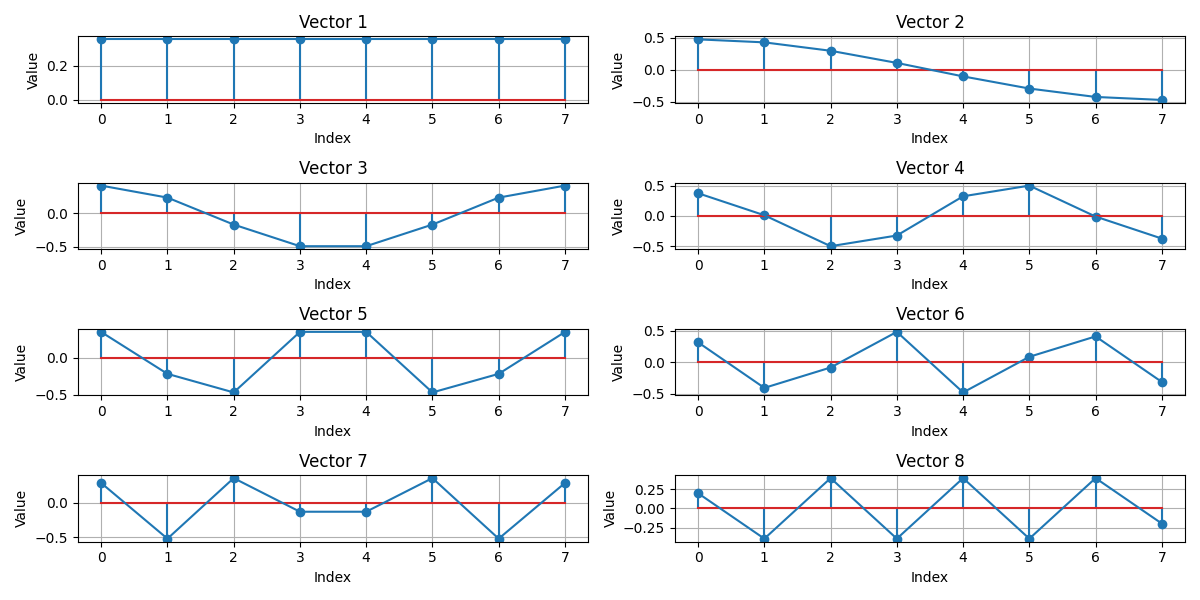
\includegraphics[scale=0.5]{CA_01Figure_3.png}
	\caption{Basis Vectors}
	\label{fig: FIG 03}
\end{figure}

\subsection{Signal Compression}
We use the formula $\bs{a}=U^T\bs{x}$ to derive:

$$\bs{a} = \begin{bmatrix} -0.0371 \\ 0.8324 \\ 0.7153 \\ 0.3991 \\ 2.0651 \\ -0.5212 \\ -1.9098 \\ -1.4373 \end{bmatrix}$$
	
In order to compress the signal we take the two largest absolute values from the vector $\bs{a}$ and create $\bs{a}_2$ with only those values and all other values replaced with 0. Since $\bs{x} = U\bs{a}$ we can use this formula to compute $\bs{x}_2 = U\bs{a}_2$. 

$$
\bs{a}_2 = \begin{bmatrix} 0 \\ 0 \\ 0 \\ 0 \\ 2.0651 \\ 0 \\ -1.9098 \\ 0  \end{bmatrix} 
\quad
\bs{x}_2 = \begin{bmatrix} 0.1540 \\ 0.5428 \\ -1.6513 \\ 0.9544 \\ 0.9544 \\ -1.6513 \\ 0.5428 \\ 0.1540 \end{bmatrix}
$$

In order to visualize the fit of $\bs{x}_2$ over $\bs{x}$. We can some of the points are very close to the original $\bs{x}$ specifically indexes 4, 6, and 8. On the other hand the approximation is inaccurate for other points. 

\begin{figure}[h!]
	\centering
	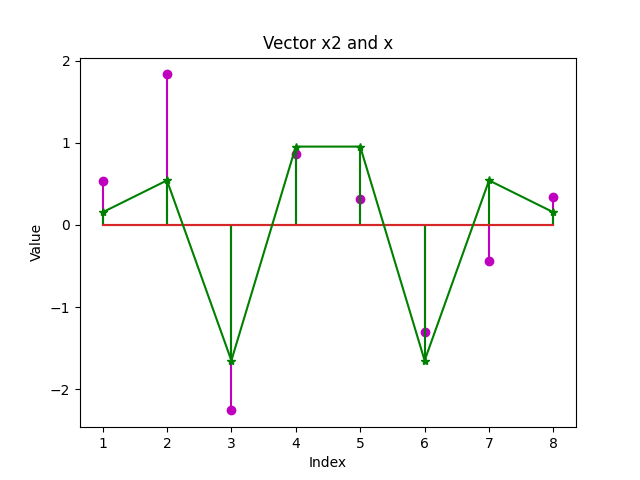
\includegraphics[scale=0.5]{CA_01Figure_4.png}
	\caption{Graphing $\bs{x}_2$ over $\bs{x}$} 
	\label{fig: FIG 04}
\end{figure}

Using the same procedure to derive $\bs{x}_4$
$$
\bs{a}_4 = \begin{bmatrix} 0 \\ 0.8324 \\ 0 \\ 0 \\ 2.0651 \\ 0 \\ -1.9098 \\ -1.4373 \end{bmatrix} 
\quad
\bs{x}_4 = \begin{bmatrix} -0.2646 \\ 1.4601 \\ -1.9704 \\ 1.6055 \\ 0.3034 \\ -1.3322 \\ -0.3745 \\ 0.0435 \end{bmatrix}
$$

\begin{figure}[h!]
	\centering
	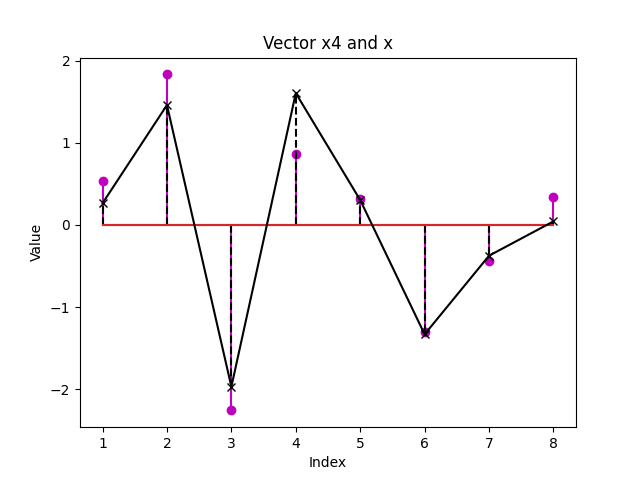
\includegraphics[scale=0.5]{CA_01Figure_5.png}
	\caption{Graphing $\bs{x}_4$ over $\bs{x}$} 
	\label{fig: FIG 05}
\end{figure}

We can see that many of the inaccuracies from $\bs{x}_2$ are no longer present in $\bs{x}_4$.

\section{Results}

We obtained the relative error between the original vector $\bs{x}$ and the compressed vectors $\bs{x}_8 = U\bs{a}$, $\bs{x}_4$, and $\bs{x}_2$.

The relative error is calculated by the equation for Root Mean Squared Error which is 
$$\sqrt{\frac{\sum_{i=1}^{n} (\bs{x} - \bs{x}_{i})^2}{\sum_{i=1}^{n} \bs{x}^2}}$$ 

We get the result that the relative error of $\bs{x}_2 = 0.5646$, $\bs{x}_4 = 0.2851$, and $\bs{x}_8 = 4.2537 \times 10^{-16}$.

As predicted, $\bs{x}_8$ has an extremely small error value since it is closest to the original signal. Consistent with the visualizations $\bs{x}_4$ has a smaller relative error than $\bs{x}_2$. By calculating the relative error we are able to determine which choice optimizes amount of data and accuracy to the signal. For example, even though $\bs{x}_8$ is the most accurate of all 3 vectors, it may be more feasible to use a compressed version that can do a similar job. In this case,  $\bs{x}_4$ appears to have a very low error despite only requiring half the data from $\bs{a}$.

\section{Summary and Conclusion}

Using DCT (Discrete Cosine Transformation) in order to compress a short audio signal we determine the best fit for the signal. We first visualized the data we had, created a matrix $U$ with column vectors that form an orthonormal basis in $\mathbb{R}^8$, and derived $\bs{a}$ where $u_1a_1+u_2a_2+...+u_8a_8=\bs{x}$. We use selective compression and choose the largest absolute values in $\bs{a}$ which should be the most influential. From there we create various visualizations and finally calculate the relative error between the compressed vectors and the original $\bs{x}$.

Based on these results we can conclude that $\bs{x}_4$ may be the best fit for the signal $\bs{x}$ that optimizes the amount of data as well as error. 

\end{document}
